\chapter{Installation des Betriebssystem}
\section{Cluster-Layout}
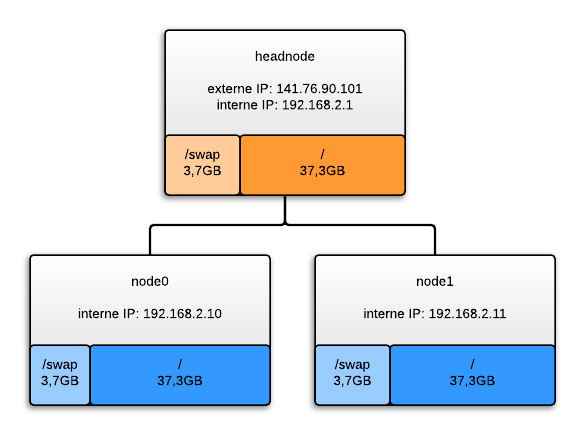
\includegraphics[width=400px]{cluster_layout.png}

/home und /shared werden exportiert.

\section{Betriebssysteminstallation}
\begin{lstlisting}[style=Bash]
# apt-get update 
# apt-get upgrade 
\end{lstlisting}
\begin{lstlisting}[style=Bash]
# adduser --geco GECO <username>
\end{lstlisting}
\begin{lstlisting}[style=Bash]
# apt-get install sudo
\end{lstlisting}
(für alle user <username>)
\begin{lstlisting}[style=Bash]
# vim /etc/sudoers
§\dotfill§
<username> ALL=(ALL)NOPASSWD:ALL
\end{lstlisting}
\begin{lstlisting}[style=Bash]
$ wget http://lctp.zih.tu-dresden.de/key/<username>.key
$ cat <username>.key >> ~.ssh/authorized_keys
\end{lstlisting}
\begin{lstlisting}[style=Bash]
# passwd -l root 
\end{lstlisting}


\section{SSH-Server}
Install SSH-Server
\begin{lstlisting}[style=Bash]
# apt-get install openssh-server 
\end{lstlisting}

\begin{lstlisting}[style=Bash]
# vim /etc/hosts.allow
§\dotfill§
sshd: 141.76.0.0/255.255.0.0
sshd: 141.30.0.0/255.255.0.0
sshd: 192.168.2.0/255.255.255.0
sshd: LOCAL 
\end{lstlisting}
\begin{lstlisting}[style=Bash]
# vim /etc/hosts.deny
§\dotfill§
sshd: ALL
\end{lstlisting}

SSH-Server konfigureren:
\begin{lstlisting}[style=Bash]
# vim /etc/ssh/sshd_config
§\dotfill§
PermitRootLogin no
RSAAuthentication yes
PubkeyAuthentication yes

AllowUsers *@141.76.*.*
AllowUsers *@141.30.*.*
AllowUsers *@192.168.2.*.*
AllowUsers *@localhost
# SSH server auf den nodes:
UseDNS no
\end{lstlisting}

Für jeden User
\begin{lstlisting}[style=Bash]
$ ssh-keygen -b 1024 -N ''
$ cat ~.ssh/id_rsa.pub >> ~./ssh/authorized_keys
\end{lstlisting}

Ein Script zur automatischen Nutzererstellung:
(dazu muss das paket whois installiert sein)
\lstinputlisting[style=Bash]{../aufgabe1/addusers.sh}

\section{Parallel Distributed Shell}
pdsh installieren
\begin{lstlisting}[style=Bash]
# apt-get install pdsh
\end{lstlisting}
/etc/genders
\begin{lstlisting}[style=Bash]
localhost headnode
node0 computenodes
\end{lstlisting}
~/.ssh/config
\begin{lstlisting}[style=Bash]
StrictHostKeyChecking no
\end{lstlisting}

\section{Git Server}
Git installieren und user git anlegen
\begin{lstlisting}[style=Bash]
# apt-get install git
# adduser git
\end{lstlisting}
configs Repo anlegen
\begin{lstlisting}[style=Bash]
# su git
# mkdir configs
# cd configs && git --bare init
\end{lstlisting}
Den ssh-key von allen usern zu /home/git/.ssh/autorized\_keys hinzufügen.
\begin{lstlisting}[style=Bash]
# su user
# ssh-keygen
# ssh-copy-id -i ~/.ssh/id\_rsa.pub git@localhost
\end{lstlisting}
Nun können alle user mit
\begin{lstlisting}[style=Bash]
# git clone git@localhost:configs
\end{lstlisting}
auf das Repository zugreifen.\\
Der etc Baum ist als submodule eingebunden. Nach dem clone muss
\begin{lstlisting}[style=Bash]
# git submodule init
# git submodule update
\end{lstlisting}
ausgeführt werden um das current\_etc Verzeichniss zu befüllen.
\subsection{etckeeper}
Installieren und konfigurieren:
\begin{lstlisting}[style=Bash]
# apt-get install etckeeper
# cd /etc && git remote add git@localhost:current_etc
\end{lstlisting}
Hook installieren sodass beim commit automatisch gepuscht wird.
/etc/.git/hooks/config
\begin{lstlisting}[style=Bash]
#!/bin/sh
git push origin master
\end{lstlisting}

\subsection{/var/log/* check in}
/var/log/* wird mit einem Script in /root/chekin\_logs.sh nach git@localhost:configs gepusht
\begin{lstlisting}[style=Bash]
#!/bin/sh
cd /root/configs
git pull
cp /var/log/* logs/ -r
git add logs/*
git commit -am "add daily logs"
git push
\end{lstlisting}
Dieses script wird per cronjob jeden Tag um 18:05 ausgeführt
\begin{lstlisting}[style=Bash]
# m h  dom mon dow   command
05 18 * * * /root/checkin_logs.sh
\end{lstlisting}
\section{BurnIn}
cpuburn und lm-sensors installieren 
\begin{lstlisting}[style=Bash]
# apt-get install cpuburn lm-sensors
\end{lstlisting}
Der BurnIn wird mit einem Script in configs/BurnIn/stresstest.sh ausgeführt.\\
burnP6 muss für jeden Core gestartet werden. Die While Schleife gibt periodisch den geparsden output von sensors mit einem Zeitstempel aus.
\begin{lstlisting}[style=Bash]
#!/bin/sh
burnP6 &
burnP6 &
`sleep 24h && killall burnP6` &

while [ "`pgrep burnP6 &>/dev/null`" ]
do
        printf "%s %s\n" "`date +%d/%m/%Y\ %H:%M:%S`" "`sensors | \
		grep C | awk -F'[:|(]' '{print $2}' | \
		grep -o '[0-9]*\.[0-9]' | cut -f1 | xargs`"
        sleep 80s
done
\end{lstlisting}
Der Test wird mit screen gestartet. Dies stellt sicher dass das Script weiterläuft wenn der ssh-user sich ausloggt.
\begin{lstlisting}[style=Bash]
# screen -dm  `./stresstest.sh > sensors.txt`
\end{lstlisting}
Die Messwerte werden mit gnuplot graphisch dargestellt.
\begin{lstlisting}[style=Bash]
#!/usr/bin/gnuplot
reset
set terminal png size 1920,1080

set xdata time
set timefmt "%d/%m/%Y %H:%M:%S"
set format x "%H:%M"
set xlabel "time"

set ylabel "Temperature in C"
set yrange [20:55]

set title "cpuburn temperature"
set key reverse Left outside
set grid
set style data linespoints

plot "sensors.txt" using 1:6 title "Core 0", \
"" using 1:7 title "Core 1"
\end{lstlisting}
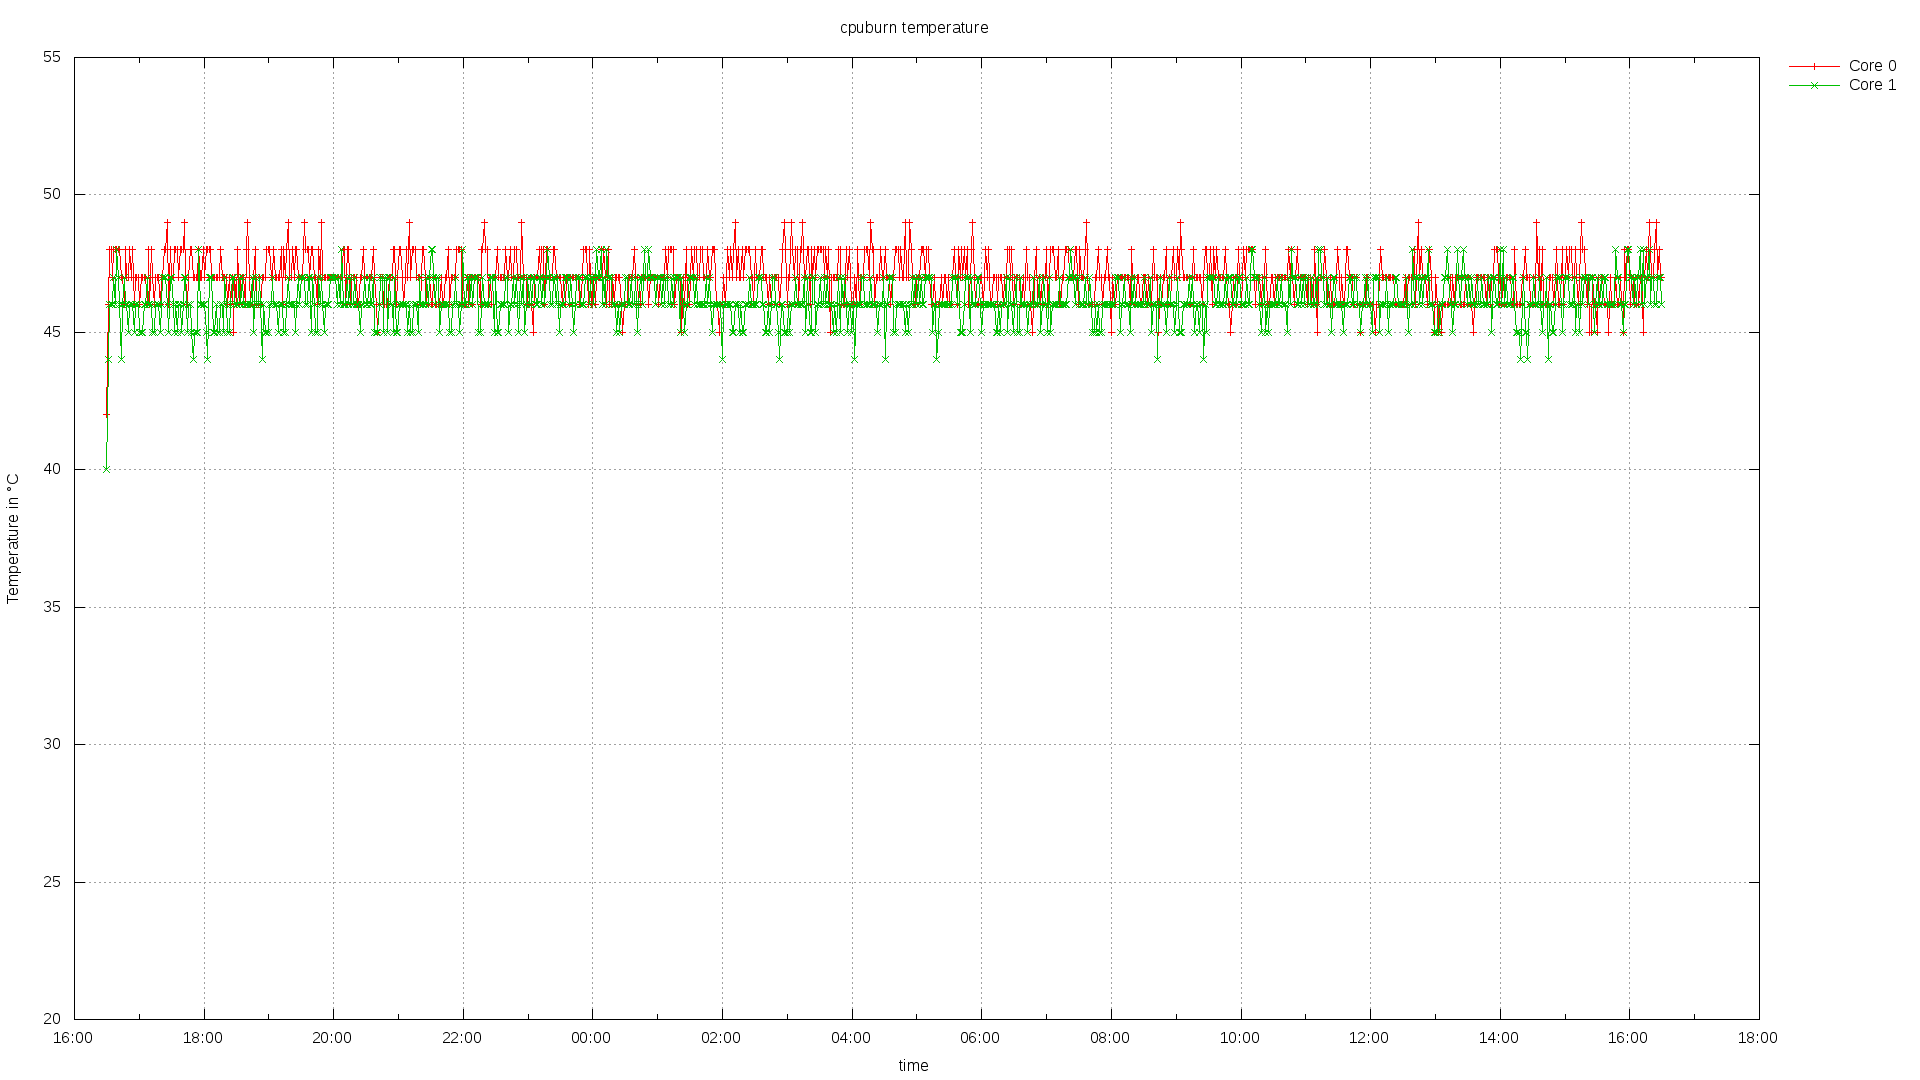
\includegraphics[width=\textwidth,height=\textheight,keepaspectratio]{../aufgabe1/BurnIn/plot.png}
